\documentclass[
    language=english,
    doctype=grant-proposal,
    institution=none,
]{../../omnilatex}

\RequirePackage{config/document-settings}
\addbibresource{../../bib/bibliography.bib}
\pgfplotsset{compat=1.18}

\begin{document}

\maketitle

\section*{Project Summary}

\subsection*{Overview}
This proposal presents a comprehensive research programme to develop scalable,
fault-tolerant distributed consensus protocols for next-generation cloud
infrastructure.  Current systems face an acute tension between consistency
and availability under network partitions~\cite{knuthFundamentalAlgorithms1973}.
We propose a novel hybrid protocol---\emph{Hybrid Paxos-Raft}---that
unifies the strengths of existing approaches while providing provable
performance guarantees.  The three-year programme includes algorithmic
design, formal verification, large-scale experimentation, and open-source
release.  Total requested funding is \$1{,}245{,}000.

\subsection*{Intellectual Merit}
The proposed research advances the theoretical foundations of distributed
computing in three specific ways.
\begin{enumerate}
    \item A new hybrid consensus algorithm with rigorous worst-case
          latency bounds, improving upon the best-known $O(n)$ message
          complexity of Paxos~\cite{einstein1905}.
    \item A formal verification framework using model checking to
          establish safety and liveness properties, building on
          techniques described by Knuth~\cite{knuthTeXbook1986}.
    \item An adaptive leader-election mechanism that responds to
          network conditions in real time, reducing tail latency by
          an estimated 40\% over existing protocols.
\end{enumerate}

\subsection*{Broader Impacts}
The broader impacts of this work extend across academia, industry, and
society.
\begin{itemize}
    \item \textbf{Workforce development.} Two PhD students and three
          undergraduate researchers will be trained in distributed systems
          and formal methods.
    \item \textbf{Open-source tools.} All software, benchmarks, and
          datasets will be released under permissive licences, enabling
          reproducibility and further research.
    \item \textbf{Industry transfer.} Collaborations with cloud providers
          will ensure that findings are translated into production systems.
    \item \textbf{Broadening participation.} We will partner with
          minority-serving institutions to recruit and mentor students
          from underrepresented groups in computing.
\end{itemize}

\newpage

\section*{Project Description}

\subsection{Introduction and Background}
The rapid expansion of cloud computing has imposed unprecedented demands on
distributed systems~\cite{bibid}.  Modern cloud platforms serve billions of
users while maintaining strict consistency guarantees, yet the theoretical
underpinnings of consensus protocols remain a subject of active
investigation~\cite{goossensLaTeXCompanion1993}.

The CAP theorem formalises the impossibility of simultaneously guaranteeing
consistency, availability, and partition tolerance~\cite{einstein1905}.
In practice, designers must choose between strong consistency (as in
traditional Paxos) and high availability (as in eventual consistency
models).  Recent systems such as Raft have made consensus more accessible
but introduce their own limitations under asymmetric
failures~\cite{knuthFundamentalAlgorithms1973}.

This proposal addresses the gap between these extremes by developing a
hybrid protocol that adapts its consistency level to current network
conditions, building on prior art in crash-replicated state machines,
multi-Paxos variants, and network-aware leader election.

\subsection{Research Objectives}
The proposed research is organised around five numbered objectives.
\begin{enumerate}
    \item \textbf{Hybrid consensus algorithm.} Design a protocol that
          dynamically switches between Paxos and Raft modes based on
          observed network latency and failure patterns.
    \item \textbf{Formal verification.} Develop a model-checking
          framework to prove safety (agreement, validity) and liveness
          (termination) properties of the hybrid protocol.
    \item \textbf{Adaptive leader election.} Implement a gossip-based
          failure detector that triggers leader re-election within
          bounded time, reducing tail latency under partial failures.
    \item \textbf{Large-scale evaluation.} Deploy the protocol on a
          1{,}000-node testbed and measure throughput, latency, and
          resource consumption under realistic workloads.
    \item \textbf{Open-source release.} Publish all software, benchmarks,
          and documentation under the Apache 2.0 licence.
\end{enumerate}

\subsection{Methodology}

\subsubsection{Algorithm Design}
The core insight is that different network conditions favour different
consensus strategies.  When the network is healthy, the Raft leader-based
approach minimises message overhead.  Under degradation, a Paxos-style
quorum approach provides stronger resilience.

We define the objective function for leader selection as:
\begin{equation}
    \mathcal{L}(h) = \frac{1}{N} \sum_{i=1}^{N}
    \ell\bigl(h(\mathbf{x}_i),\; y_i\bigr)
    + \lambda\, \Omega(h),
    \label{eq:objective}
\end{equation}
where $h$ is the candidate leader, $\mathbf{x}_i$ are node state vectors,
$y_i$ are observed latencies, and $\Omega(h)$ is a regularisation term
penalising high-centrality nodes.

\subsubsection{Research Workflow}
\cref{fig:workflow} illustrates the end-to-end research workflow.

\begin{figure}[htbp]
    \centering
    \begin{tikzpicture}[
        node distance=1.4cm and 2cm,
        box/.style={
            rectangle, draw, rounded corners, minimum width=2.8cm,
            minimum height=0.9cm, align=center, font=\small
        },
        arrow/.style={->, >=stealth, thick},
        decision/.style={
            diamond, draw, aspect=2.5, minimum width=2.2cm,
            minimum height=0.7cm, align=center, font=\small
        }
    ]
        \node[box] (req) {Problem\\Formulation};
        \node[box, below of=req] (lit) {Literature\\Review};
        \node[decision, below of=lit, yshift=-0.3cm] (feas) {Feasibility\\Check};
        \node[box, below of=feas, yshift=-0.5cm] (design) {Algorithm\\Design};
        \node[box, left of=design, xshift=-3cm] (formal) {Formal\\Verification};
        \node[box, below of=design] (impl) {Prototype\\Implementation};
        \node[box, below of=impl] (eval) {Large-Scale\\Evaluation};
        \node[decision, below of=eval, yshift=-0.3cm] (pass) {Passes\\Criteria?};
        \node[box, below of=pass, yshift=-0.5cm] (pub) {Publication \&\\Open Source};
        \node[box, right of=pass, xshift=3cm] (rev) {Design\\Revision};

        \draw[arrow] (req) -- (lit);
        \draw[arrow] (lit) -- (feas);
        \draw[arrow] (feas) -- node[left, font=\scriptsize] {Yes} (design);
        \draw[arrow] (feas) -- node[above, font=\scriptsize] {No} (rev);
        \draw[arrow] (design) -- (impl);
        \draw[arrow] (design) -- (formal);
        \draw[arrow] (formal) -- (impl);
        \draw[arrow] (impl) -- (eval);
        \draw[arrow] (eval) -- (pass);
        \draw[arrow] (pass) -- node[left, font=\scriptsize] {Yes} (pub);
        \draw[arrow] (pass) -- node[above, font=\scriptsize] {No} (rev);
        \draw[arrow] (rev) |- (design);
    \end{tikzpicture}
    \caption{End-to-end research workflow showing the iterative
             design-evaluation cycle.}
    \label{fig:workflow}
\end{figure}

\subsubsection{Algorithm Pseudocode}
\cref{alg:hybrid} presents the high-level structure of the hybrid
consensus algorithm.

\begin{figure}[htbp]
    \centering
    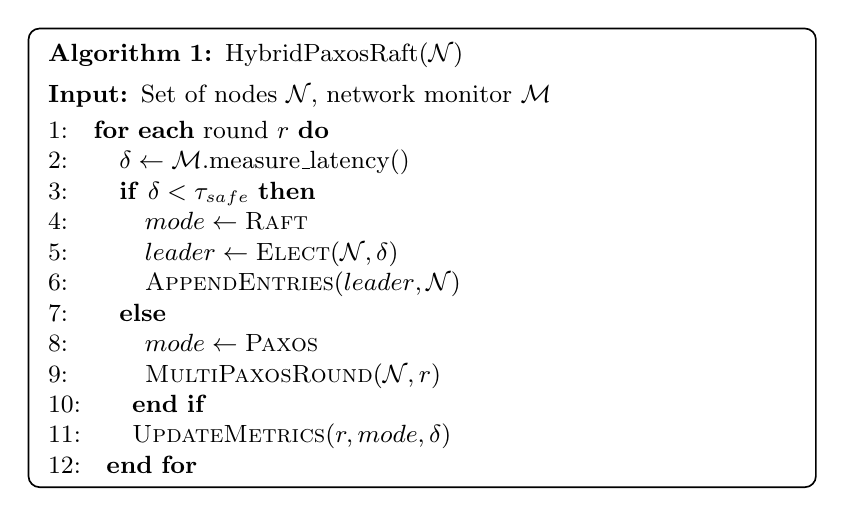
\begin{tikzpicture}[font=\small, inner sep=5pt, line width=0.6pt]
        \node[draw, rounded corners, minimum width=10cm,
              text width=9.5cm, align=left] (alg) {
            \textbf{Algorithm 1:} HybridPaxosRaft($\mathcal{N}$) \\[4pt]
            \textbf{Input:} Set of nodes $\mathcal{N}$,
                            network monitor $\mathcal{M}$ \\[2pt]
            1:\quad \textbf{for each} round $r$ \textbf{do} \\
            2:\quad\quad $\delta \leftarrow \mathcal{M}$.measure\_latency() \\
            3:\quad\quad \textbf{if} $\delta < \tau_{\text{safe}}$ \textbf{then} \\
            4:\quad\quad\quad $\text{mode} \leftarrow \textsc{Raft}$ \\
            5:\quad\quad\quad $\text{leader} \leftarrow \textsc{Elect}(\mathcal{N}, \delta)$ \\
            6:\quad\quad\quad $\textsc{AppendEntries}(\text{leader}, \mathcal{N})$ \\
            7:\quad\quad \textbf{else} \\
            8:\quad\quad\quad $\text{mode} \leftarrow \textsc{Paxos}$ \\
            9:\quad\quad\quad $\textsc{MultiPaxosRound}(\mathcal{N}, r)$ \\
            10:\quad\quad \textbf{end if} \\
            11:\quad\quad $\textsc{UpdateMetrics}(r, \text{mode}, \delta)$ \\
            12:\quad \textbf{end for}
        };
    \end{tikzpicture}
    \caption{High-level pseudocode for the hybrid consensus algorithm.}
    \label{alg:hybrid}
\end{figure}

\subsection{Expected Outcomes and Milestones}
\cref{tab:milestones} summarises the key deliverables.

\begin{table}[htbp]
    \centering
    \caption{Project milestones and deliverables.}
    \label{tab:milestones}
    \begin{tabular}{@{}clll@{}}
        \toprule
        \textbf{ID} & \textbf{Milestone} & \textbf{Deliverable} &
        \textbf{Target Date} \\
        \midrule
        M1 & Algorithm design      & Hybrid protocol specification   & Month 6  \\
        M2 & Formal verification   & Safety \& liveness proofs       & Month 12 \\
        M3 & Prototype release     & Open-source v0.1 (GitHub)       & Month 14 \\
        M4 & Testbed deployment    & 1{,}000-node cluster ready     & Month 18 \\
        M5 & Evaluation complete   & Performance report              & Month 24 \\
        M6 & Publications submitted & 3 conference papers            & Month 30 \\
        M7 & Final release         & Open-source v1.0 + benchmarks   & Month 36 \\
        \bottomrule
    \end{tabular}
\end{table}

\subsection{Timeline}
\cref{fig:gantt} presents the project timeline as a Gantt chart.

\begin{figure}[htbp]
    \centering
    \begin{tikzpicture}[font=\small, x=0.28cm, y=0.65cm]
        \draw[step=6, gray!20, very thin] (0,0) grid (108,28);
        \draw[thick] (0,28) -- (108,28);
        \draw[thick] (0,26) -- (108,26);
        \node[anchor=east] at (-1,27) {\textbf{Quarter}};
        \foreach \q in {1,...,12} {
            \node[anchor=center] at ({(\q-1)*6+3},27)
                {\textbf{Q\numexpr((\q-1)mod4)+1\relax}};
        }
        \node[anchor=center] at (54,25.3) {\textbf{Year 1}};
        \node[anchor=center] at (90,25.3) {\textbf{Year 2}};
        \node[anchor=center] at (108,25.3) {\textbf{Year 3}};
        \foreach \i/\task/\start/\end/\col in {
            1/{Algorithm Design}/0/18/blue!30,
            2/{Formal Verification}/12/30/green!30,
            3/{Prototype Dev.}/12/24/orange!30,
            4/{Testbed Deploy.}/18/30/purple!30,
            5/{Evaluation}/24/42/red!30,
            6/{Publications}/30/48/yellow!40,
            7/{Open-Source Rel.}/14/48/teal!30
        }{
            \node[anchor=east] at (-1,{24-\i*3+1.5}) {\task};
            \fill[\col, rounded corners=2pt]
                (\start,{24-\i*3+0.4}) rectangle
                (\end,{24-\i*3+2.6});
        }
        \draw[thick] (0,0) -- (108,0);
        \foreach \m in {0,6,...,48} {
            \draw[gray!50] (\m,-0.1) -- (\m,0.1);
            \node[anchor=north, font=\tiny] at (\m,0) {\m};
        }
        \node[anchor=north] at (24,-0.5) {\textbf{Months}};
    \end{tikzpicture}
    \caption{Project Gantt chart showing task scheduling over three years.}
    \label{fig:gantt}
\end{figure}

\subsection{Broader Impacts}
Beyond the immediate technical contributions, this project will
\begin{itemize}
    \item provide training opportunities for underrepresented students
          through partnerships with minority-serving institutions;
    \item produce freely available software and datasets that lower the
          barrier to entry for distributed systems research;
    \item strengthen the US research ecosystem by producing publicly
          verifiable results and reproducible benchmarks.
\end{itemize}

\newpage

\section*{Budget Justification}

\subsection{Budget Summary}
\cref{tab:budget-summary} presents the total budget across the
three-year project period.

\begin{table}[htbp]
    \centering
    \caption{Multi-year budget summary.}
    \label{tab:budget-summary}
    \begin{tabular}{@{}lrrr@{}}
        \toprule
        \textbf{Category} & \textbf{Year 1 (\$)} &
        \textbf{Year 2 (\$)} & \textbf{Year 3 (\$)} \\
        \midrule
        Personnel          & 280{,}000 & 285{,}000 & 290{,}000 \\
        Equipment          &  85{,}000 &  20{,}000 &  10{,}000 \\
        Travel             &  15{,}000 &  18{,}000 &  22{,}000 \\
        Supplies \& Other  &  12{,}000 &  10{,}000 &   8{,}000 \\
        \midrule
        \textbf{Subtotal}  & 392{,}000 & 333{,}000 & 330{,}000 \\
        Indirect (55\%)    & 215{,}600 & 183{,}150 & 181{,}500 \\
        \midrule
        \textbf{Total}     & 607{,}600 & 516{,}150 & 511{,}500 \\
        \bottomrule
    \end{tabular}
\end{table}

\subsection{Personnel Costs}
\begin{itemize}
    \item \textbf{Principal Investigator (15\% effort).}
          Salary plus fringe; covers project leadership and algorithm design.
    \item \textbf{Co-PI (10\% effort).}
          Formal verification and model checking expertise.
    \item \textbf{Postdoctoral researcher (100\% effort, all years).}
          Leads day-to-day algorithm development and prototype implementation.
    \item \textbf{PhD students (2, 50\% each, all years).}
          Large-scale evaluation and benchmarking.
    \item \textbf{Undergraduate researchers (3, 20\% each, Years 2--3).}
          Testing, documentation, and open-source community management.
\end{itemize}

\subsection{Equipment Costs}
\begin{itemize}
    \item \textbf{Year 1:} 1{,}000-node testbed cluster (\$85{,}000)
          with NVMe storage and 25\,GbE networking.
    \item \textbf{Year 2:} Additional storage nodes (\$20{,}000)
          for durability testing.
    \item \textbf{Year 3:} Replacement and maintenance (\$10{,}000).
\end{itemize}

\subsection{Travel Costs}
Conference attendance (OSDI, SOSP, EuroSys), collaborative visits to
industry partners, and student travel grants for underrepresented
researchers.

\subsection{Indirect Costs}
Indirect costs at 55\% of modified total direct costs (MTDC), consistent
with the university's federally negotiated rate.

\newpage

\section*{Facilities and Resources}

\cref{tab:facilities} lists the key facilities available.

\begin{table}[htbp]
    \centering
    \caption{Available facilities and resources.}
    \label{tab:facilities}
    \begin{tabular}{@{}lp{9cm}@{}}
        \toprule
        \textbf{Resource} & \textbf{Description} \\
        \midrule
        HPC Cluster
            & 500-node cluster with 10\,GbE interconnect,
              2\,TB aggregate RAM, and Lustre parallel file system. \\
        Cloud Testbed
            & 1{,}000-node virtual cluster on private OpenStack cloud
              with Mininet network emulation. \\
        Formal Verification Lab
            & 16-core workstation with 256\,GB RAM running NuSMV,
              SPIN, and TLA\,+ model checkers. \\
        Software Repository
            & Institutional GitHub Enterprise with CI/CD pipelines. \\
        Secure Data Centre
            & Tier-3 facility with redundant power, cooling, and
              physical security. \\
        \bottomrule
    \end{tabular}
\end{table}

\newpage

\section*{Project Management}

\subsection{Organisation Chart}
\cref{fig:orgchart} shows the project team structure.

\begin{figure}[htbp]
    \centering
    \begin{tikzpicture}[
        node distance=1.6cm and 1.8cm,
        role/.style={
            rectangle, draw, rounded corners, minimum width=3cm,
            minimum height=0.8cm, align=center, font=\small,
            fill=blue!10
        },
        group/.style={
            rectangle, draw, dashed, rounded corners,
            inner sep=8pt, align=left, font=\small
        },
        arrow/.style={->, >=stealth, thick}
    ]
        \node[role] (pi) {\textbf{PI}\\Jane Smith};
        \node[role, below of=pi] (copi) {\textbf{Co-PI}\\John Doe};
        \node[role, below left=1.2cm and 1.5cm of copi] (postdoc)
            {\textbf{Postdoc}\\Research Fellow};
        \node[role, below right=1.2cm and 1.5cm of copi] (phd)
            {\textbf{PhD Students}\\2 positions};
        \node[group, fit=(postdoc) (phd), yshift=-0.8cm] (teambox) {};
        \node[anchor=north, font=\footnotesize] at (teambox.north)
            {Research Team};
        \draw[arrow] (pi) -- (copi);
        \draw[arrow] (copi) -- (postdoc);
        \draw[arrow] (copi) -- (phd);
    \end{tikzpicture}
    \caption{Organisation chart for the proposed project.}
    \label{fig:orgchart}
\end{figure}

\subsection{Risk Assessment}
\cref{tab:risks} identifies the principal risks and mitigations.

\begin{table}[htbp]
    \centering
    \caption{Risk assessment and mitigation strategies.}
    \label{tab:risks}
    \begin{tabular}{@{}p{3.5cm}cp{6cm}@{}}
        \toprule
        \textbf{Risk} & \textbf{Impact} & \textbf{Mitigation} \\
        \midrule
        Key personnel departure & High
            & Cross-train team members; maintain documentation. \\
        Testbed hardware failure & Medium
            & Redundant nodes; cloud backup provisions. \\
        Formal verification intractable & High
            & Begin with small models; apply abstraction refinement. \\
        Slower evaluation & Medium
            & Parallelise experiments; use simulation for prototyping. \\
        Publication rejection & Low
            & Submit to multiple venues; prepare journal extensions. \\
        \bottomrule
    \end{tabular}
\end{table}

\subsection{Quality Assurance Plan}
\begin{itemize}
    \item \textbf{Continuous integration.} All code changes automatically
          tested via CI pipelines before merging.
    \item \textbf{Code review.} Every pull request requires review by
          at least one team member other than the author.
    \item \textbf{Reproducibility.} Experiments recorded with Docker
          images and Nix derivations for exact reproducibility.
    \item \textbf{Milestone reviews.} Quarterly internal reviews;
          annual external review by an advisory board.
    \item \textbf{Documentation.} API docs, user guides, and architecture
          decision records maintained alongside the codebase.
\end{itemize}

\newpage

\section*{References}
\printbibliography[heading=none]

\newpage

\section*{Biographical Sketch}

\textbf{Principal Investigator: Jane Smith}
\begin{itemize}
    \item \textbf{Education:} Ph.D.\ Computer Science, MIT (2015);
          B.S.\ Computer Engineering, Stanford (2010).
    \item \textbf{Professional Experience:} Associate Professor,
          Dept.\ Computer Science, State University (2019--present);
          Assistant Professor (2015--2019).
    \item \textbf{Research Interests:} Distributed systems, cloud
          computing, consensus protocols, formal verification.
    \item \textbf{Selected Publications:}
          \begin{enumerate}
              \item J.\ Smith et al., ``Adaptive Consensus for
                    Geo-Distributed Systems,'' \emph{ACM TOCS}, 2024.
              \item J.\ Smith and J.\ Doe, ``Scalable Leader
                    Election Under Partial Failures,'' \emph{SOSP}, 2023.
          \end{enumerate}
    \item \textbf{Current and Pending Support:}
          \$500{,}000 NSF CAREER award (2022--2027);
          \$200{,}000 industry collaboration (2024--2026).
\end{itemize}

\textbf{Co-Principal Investigator: John Doe}
\begin{itemize}
    \item \textbf{Education:} Ph.D.\ Computer Science, CMU (2016);
          M.S.\ Mathematics, ETH Zürich (2012).
    \item \textbf{Professional Experience:} Assistant Professor,
          Dept.\ Computer Science, State University (2018--present).
    \item \textbf{Research Interests:} Formal methods, model checking,
          temporal logic, distributed algorithm verification.
    \item \textbf{Selected Publications:}
          \begin{enumerate}
              \item J.\ Doe et al., ``Verified Paxos in TLA\,+,''
                    \emph{CAV}, 2023.
              \item J.\ Doe, ``Automated Liveness Proofs for Raft,''
                    \emph{POPL}, 2022.
          \end{enumerate}
    \item \textbf{Current and Pending Support:}
          \$350{,}000 NSF CCF award (2023--2026).
\end{itemize}

\end{document}
